
\documentclass[12pt,a4paper]{article}

\usepackage{amsmath}
\usepackage{graphicx}
\usepackage{xcolor}
\usepackage{colortbl}
\usepackage{array}
\usepackage{float}
\usepackage{caption}
\usepackage{geometry}

\geometry{margin=1in}
\setlength{\emergencystretch}{3em}

\definecolor{custompurple}{RGB}{200,20,200}
\colorlet{customorange}{red!60!yellow}

\begin{document}
	
	\begin{center}
		{\LARGE \textbf{Assignment 4}}\\[5pt]
		{\large Lists, Colors, Figures etc.}\\[5pt]
		TW Lab 2025
	\end{center}
	
	\section{Lists}
	
	Following are some technologies that can be used to format content:
	
	\begin{itemize}
		\item \LaTeX
		\item HTML (+CSS)
		\item Markdown
	\end{itemize}
	
	You would most likely use \LaTeX\ in the following scenarios:
	
	\begin{enumerate}
		\item To write research papers
		\item To embed math equations within other software (e.g. GDocs, HTML etc.)
		\item To create your CV, project reports \& presentations
	\end{enumerate}
	
	There are three main categories of electronic markup:
	
	\begin{description}
		\item[Presentational] Used by traditional word-processing systems: binary codes embedded within document text that produce the WYSIWYG (``what you see is what you get'') effect. e.g. Microsoft Word.
		
		\item[Procedural] Markup is embedded in text which provides instructions for programs to process the text. e.g. TEX.
		
		\item[Descriptive] Markup is specifically used to label parts of the document for what they are, rather than how they should be processed. e.g. \LaTeX, HTML5.
	\end{description}
	
	\section{Tables \& Colors}
	
	Code for Table 1 is written in this subsection. However, it will be rendered on a special page.
	
	\begin{table}[p]
		\centering
		\caption{This table should be rendered on a special page.}
		\label{tab:languages}
		
		\renewcommand{\arraystretch}{1.5}
		
		\begin{tabular}{
				|>{\raggedright\arraybackslash}p{2.5cm}
				|>{\centering\arraybackslash}p{2cm}
				|>{\centering\arraybackslash}p{2cm}
				|>{\raggedright\arraybackslash}p{3.5cm}|
			}
			\hline
			\textbf{Language} &
			\textbf{Requires compilation} &
			\textbf{Output} &
			\textbf{Use}\\
			\hline
			C/C++ & Yes & Executable & To make apps\\
			\hline
			\LaTeX & Yes & PDF & To make documents\\
			\hline
			HTML/CSS/JS & No & Webpage & To make websites\\
			\hline
		\end{tabular}
		
		\vspace{5mm}
		
		\begin{tabular}{|c|c|c|c|}
			\hline
			2.5 cm & 2 cm & 2 cm & 3.5 cm\\
			\hline
		\end{tabular}
		
	\end{table}
	
	\clearpage
	
	Read more about how colors are represented as numbers.
	
	The custom color is defined using RGB values:
	
	\[
	\text{RGB}=(200,20,200)
	\]
	
	Its HTML hexadecimal notation is:
	
	\[
	\texttt{\#C814C8}
	\]
	
	Another custom color is created using \verb|\colorlet| with 60\% red and 40\% yellow.
	
	The following equation uses both custom colors:
	
	\[
	\textcolor{custompurple}{T(n)}
	=
	\textcolor{customorange}{aT(n/b)+f(n)}
	\]
	
	The table placement options are:
	
	\begin{itemize}
		\item \texttt{[t]} -- Top of page
		\item \texttt{[b]} -- Bottom of page
		\item \texttt{[h]} -- Approximately here
		\item \texttt{[p]} -- Special page containing floats
	\end{itemize}
	
	\section{Figures}
	
	\subsection{Pictures: Rotation \& Cropping}
	
	Include the MNIT logo and rotate it appropriately.
	
	\begin{figure}[htbp]
		\centering
		\includegraphics[
		width=0.3\textwidth,
		angle=90
		]{mnit_logo.png}
		\caption{MNIT logo}
		\label{fig:mnit-logo}
	\end{figure}
	
	Include the MNIT building picture, crop the sky and make it as wide as the text.
	
	\begin{figure}[htbp]
		\centering
		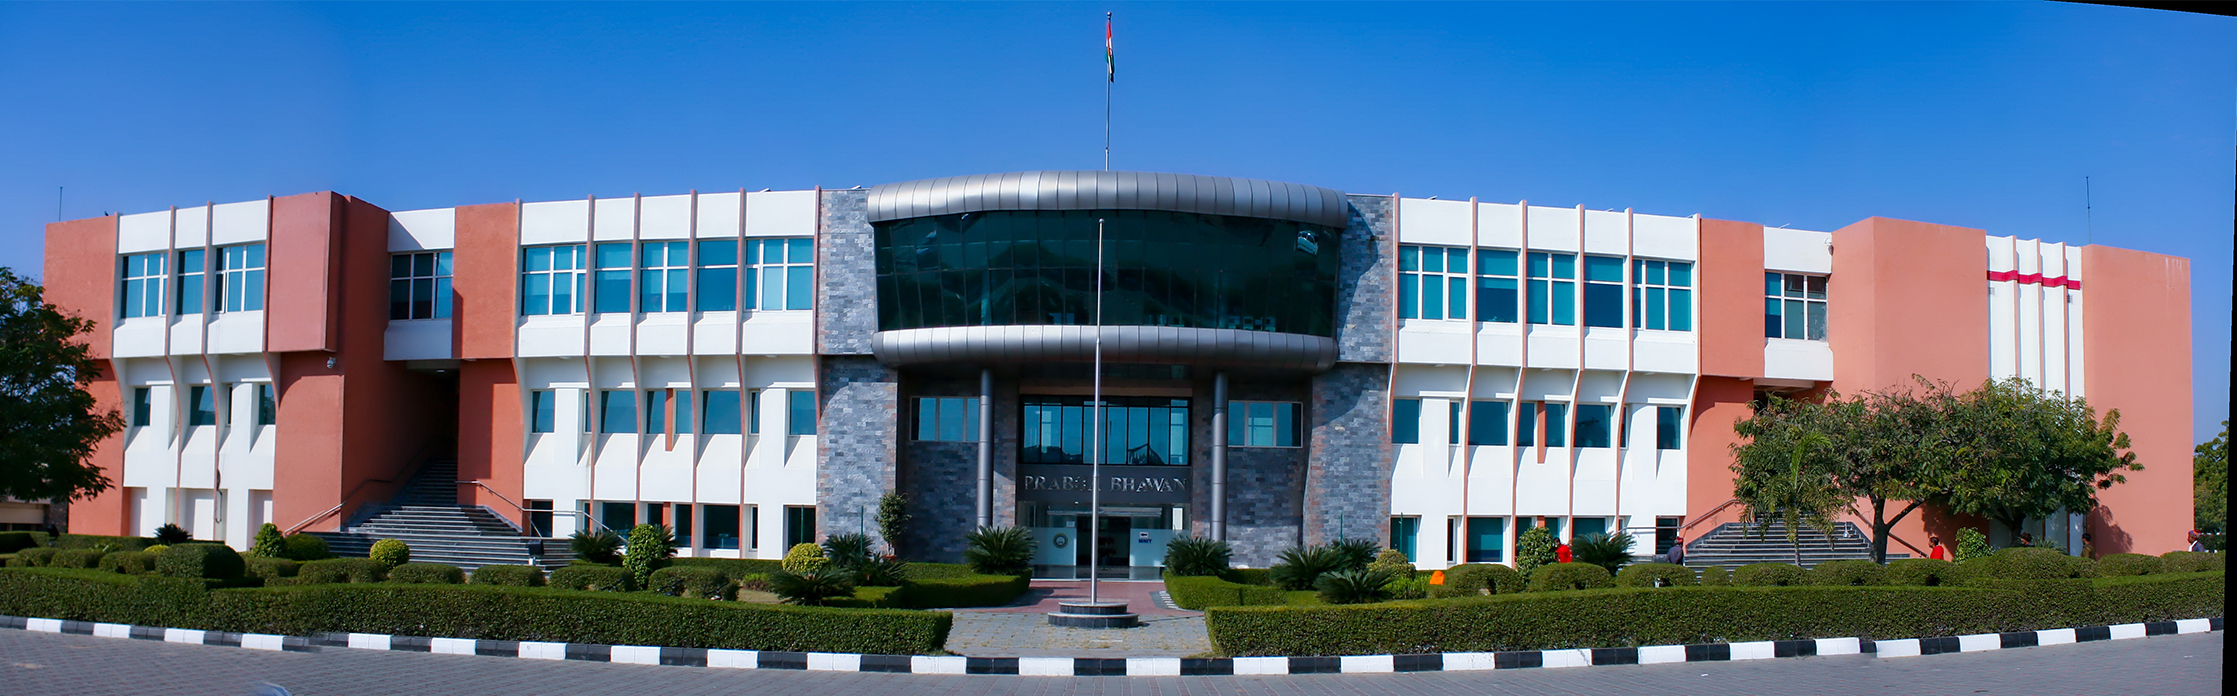
\includegraphics[
		width=\textwidth,
		height=5cm,
		keepaspectratio,
		trim=0 0 0 1.5cm,
		clip
		]{mnit_building.jpg}
		\caption{This is a floating image and can appear anywhere.}
		\label{fig:mnit-building}
	\end{figure}
	
	\subsection{Multiple Images}
	
	This subsection includes two minipages with equal width.
	
	\begin{figure}[htbp]
		\centering
		
		\begin{minipage}[c]{0.48\textwidth}
			\centering
			\includegraphics[
			width=0.95\linewidth
			]{mnit_logo.png}
			\captionof{figure}{This is the first minipage}
			\label{fig:first-minipage}
		\end{minipage}
		\hfill
		\begin{minipage}[c]{0.48\textwidth}
			\centering
			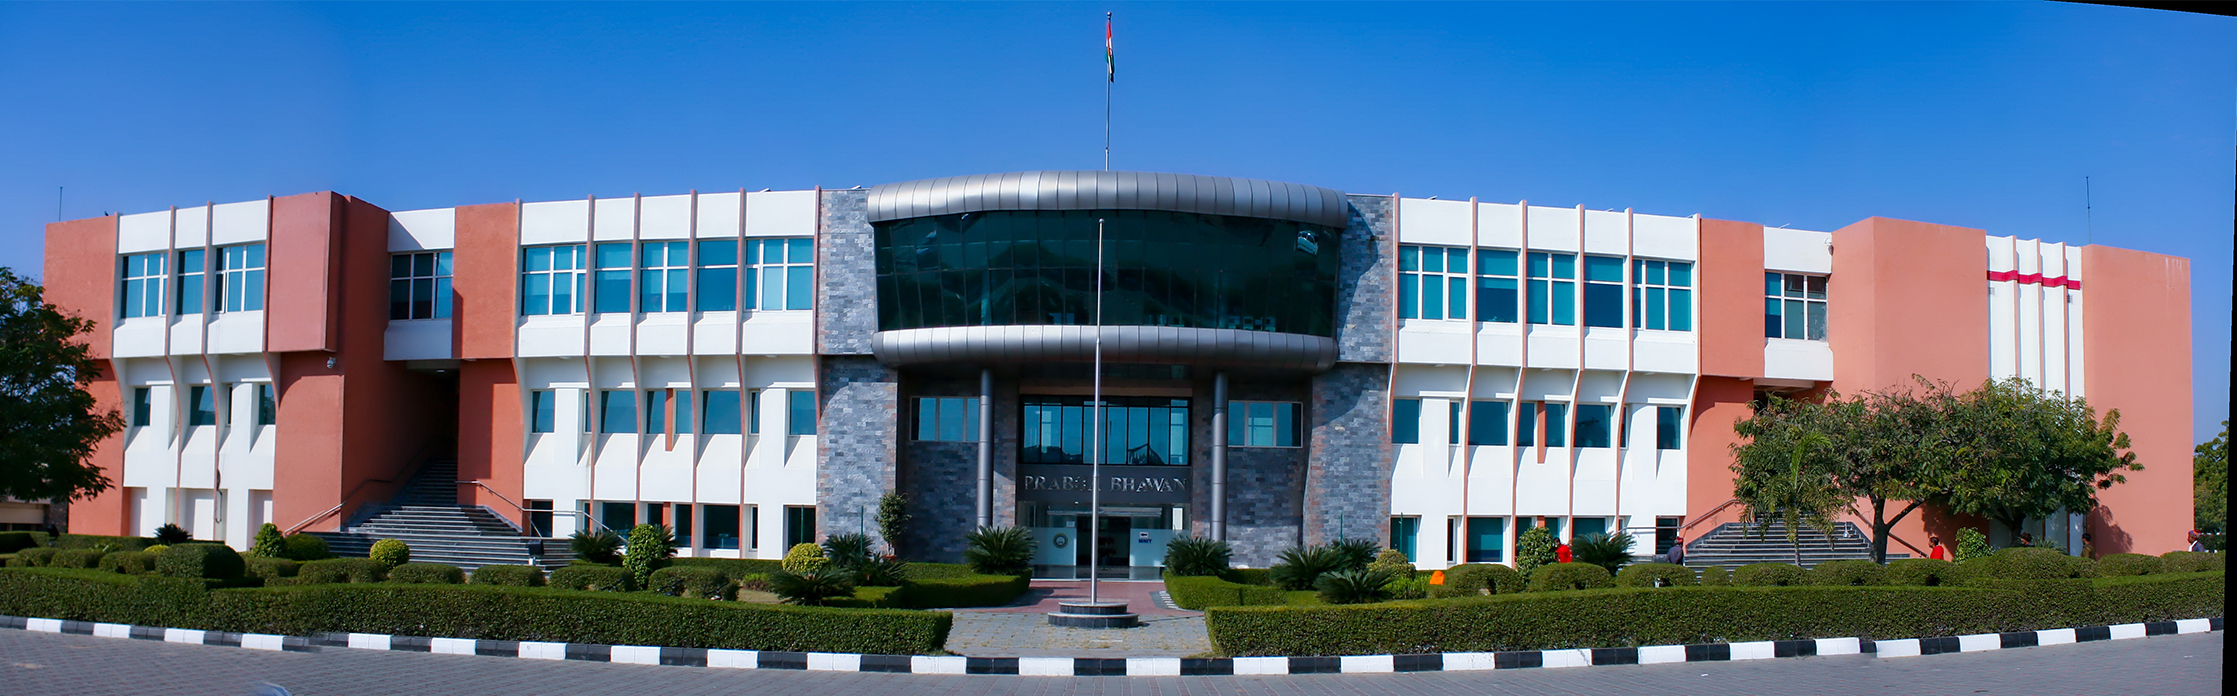
\includegraphics[
			width=0.95\linewidth
			]{mnit_building.jpg}
			\captionof{figure}{This is the second minipage}
			\label{fig:second-minipage}
		\end{minipage}
		
	\end{figure}
	
\end{document}
